\documentclass[12pt,a4paper]{article} %wielkość czcionki i papieru
\usepackage[margin=2cm,headheight=0pt,includeheadfoot]{geometry}
%\usepackage{geometry}
%\usepackage[margin=2cm]{geometry}
\usepackage{amssymb}
%\usepackage[polish]{babel} %język polski
\usepackage[utf8]{inputenc} %interpretacja znaków
\usepackage[T1]{fontenc} %interpretacja polskich znaków
\usepackage{lmodern} 
%\usepackage[]{natbib} %bibliografia
\usepackage{graphicx} %wstawianie obrazów i do tablicy
\usepackage{wrapfig} %obrazy przyległe do tekstu
%\usepackage{mathtools}  %funkcje matematyczne
%\mathtoolsset{showonlyrefs} %nienumerowanie wzorów matematycznych
\usepackage{amsmath}
\usepackage{float}
\usepackage{booktabs} % do tablicy
\usepackage{multirow} % do tablicy
\usepackage{enumitem}  % tryb listy [pogrubiony tekst] [wyjasnienie] 
\usepackage[font=small]{caption} % podpisy małe
\usepackage[font=small]{subcaption} % subpodpisy małe
\usepackage[pdftex,hidelinks]{hyperref} % href, ukrywa czerwone obwódki wokół linków
\usepackage[table,xcdraw]{xcolor}
\usepackage{lscape}
\pagestyle{plain} % zwykły tekst
\usepackage{listings}
\usepackage{lscape}
% \pagenumbering{gobble}
%\usepackage[framed,numbered,autolinebreaks,useliterate]{mcode} %matlab
%\usepackage{gensymb} %degree w mathmode

\lstset{
	basicstyle=\ttfamily,        % the size of the fonts that are used for the code
	breakatwhitespace=false,         % sets if automatic breaks should only happen at whitespace
  	breaklines=true,                 % sets automatic line breaking
  	frame=single,	                 % adds a frame around the code
  	numbers=left,                    % where to put the line-numbers; possible values are (none, left, right)
  	numbersep=5pt,                   % how far the line-numbers are from the code
  	numberstyle=\tiny,					 % the style that is used for the line-numbers
  	tabsize=2,	                   % sets default tabsize to 2 spaces
}

%-------------------------------------------------------------------------
%nagłówek i stopka


%-------------------------------------------------------------------
% O dokumencie
\title{Aritificial Intelligence and Machine Learning --- MDP, Q-learning}
%\author{Piotr Matuszak}


\begin{document}

\begin{center}
\begin{LARGE}
\vspace{-40pt}
Aritificial Intelligence and Machine Learning --- MDP, Q-learning
\end{LARGE}
\vspace{10pt}

Piotr Matuszak 218582
\end{center}

\vspace{20pt}

\section{Running the program}

\textbf{Requirements:} \texttt{Python 3.7}  or higher, \texttt{gnuplot}

\noindent\textbf{Installing prerequisities:} \texttt{pip install -r requirements.txt}

\subsection{Running a program}

\begin{itemize}
\item File \texttt{mdp\_run.py} will generate all results described in section \ref{sec_mdp} of this report. All files for \texttt{gnuplot} to generate plots will be put in \texttt{results/} directory. Plots are also automatically generated in this directory.
\item File \texttt{qlearning\_run.py} will print all results described in section \ref{sec_qlearn} of this report.
\item To redraw a plot from provided output file (in \texttt{results/} directory), run: \texttt{./plotter.sh filename}. Plot will be generated under a name \texttt{filename.png}.
\item Worlds are defined in \texttt{toml} format in \texttt{worlds/} directory.
\end{itemize}

\section{Markov Decision Problem}\label{sec_mdp}

\subsection{World 1}

First world is defined in \texttt{worlds/default.toml} file. It is a 4x3 world as defined in the task description\footnote{\url{http://zpcir.ict.pwr.wroc.pl/~witold/ai/MDPRL_assignment.html}}. Termination value of $0.0001$ stopped the calculation of utilities at 15th iteration.

\begin{lstlisting}[caption={Results of MDP utility value calculation for 4x3 world. Upper left corner of each field describes the policy, upper right - type of the field (S - start, N - normal, F - forbidden, T - terminal), bottom - utility value.}]
---------------------------------
|>     N|>     N|>     N|x     T|
|0.81155|0.86780|0.91780|      1|
---------------------------------
|^     N|x     F|^     N|x     T|
|0.76155|xxxxxxx|0.66027|     -1|
---------------------------------
|^     S|<     N|<     N|<     N|
|0.70528|0.65526|0.61137|0.38787|
---------------------------------
\end{lstlisting}

\begin{figure}[H]
\centering
	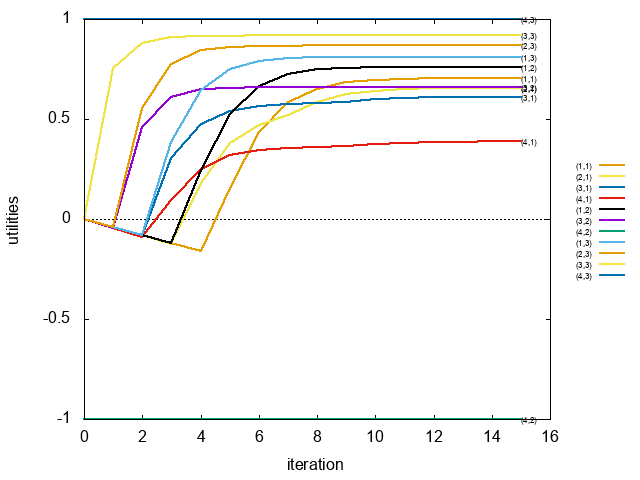
\includegraphics[width=0.8\textwidth]{../results/default.png}
	\caption{Convergence plot for 4x3 world}
	\label{w1}
\end{figure}


\subsection{World 2}

Second world is defined in \texttt{worlds/default2.toml} as defined in aforementioned task description. It is a 4x4 world. Termination value of $0.0001$ stopped the calculation of utilities at 20th iteration.


\begin{lstlisting}[caption={Results of MDP utility value calculation for 4x4 world. Field marked as B is a special field.}]
---------------------------------
|>     N|>     N|>     N|v     N|
|81.9383|84.2609|86.5860|88.8827|
---------------------------------
|>     N|>     N|>     N|v     N|
|81.7354|84.2724|87.0595|91.5547|
---------------------------------
|^     N|^     N|>     B|v     N|
|79.5935|80.5997|70.4670|94.5352|
---------------------------------
|^     S|^     N|x     F|x     T|
|77.4525|78.2494|xxxxxxx|    100|
---------------------------------
\end{lstlisting}

It can be noticed that special field is avoided due to its high penalty.

\begin{figure}[H]
\centering
	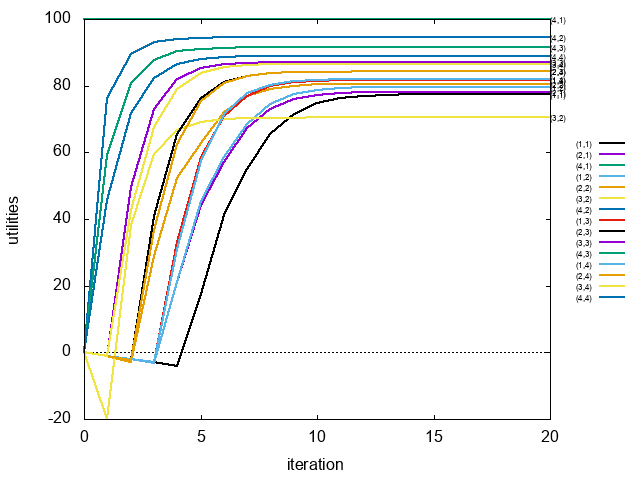
\includegraphics[width=0.8\textwidth]{../results/default2.png}
	\caption{Convergence plot for 4x4 world}
	\label{q2}
\end{figure}

\subsection{World 2 with modifications -- reward}

In this task, utility values were modified in the following way:
\begin{itemize}
	\item default reward is $-10$ instead of $-1$
	\item special field has reward $-1$ instead of $-20$.
\end{itemize}
This was defined in a file \texttt{worlds/default3.toml}.
\begin{lstlisting}[caption={Results of MDP utility value calculation for 4x4 world, modified reward}]
---------------------------------
|>     N|>     N|v     N|v     N|
|29.6567|41.3267|52.9342|57.7182|
---------------------------------
|>     N|>     N|v     N|v     N|
|40.3029|53.6510|67.0818|71.6713|
---------------------------------
|>     N|>     N|>     B|v     N|
|49.2453|64.9589|81.6602|85.7762|
---------------------------------
|>     S|^     N|x     F|x     T|
|38.4636|50.2279|xxxxxxx|    100|
---------------------------------
\end{lstlisting}

In this situation, special field starts to "attract" the policies around, because it is better to pass through this field than any other (it has less of a negative reward than all normal fields). Nevertheless, the high reward of terminal state makes policies to point towards it.

\begin{figure}[H]
\centering
	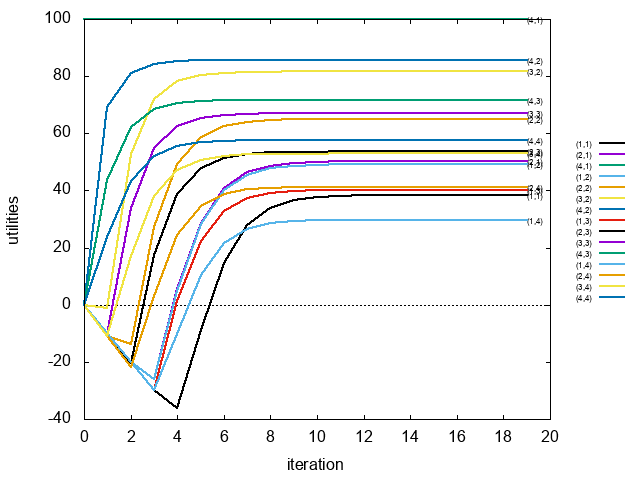
\includegraphics[width=0.8\textwidth]{../results/default3.png}
	\caption{Convergence plot for 4x4 world, modified reward}
	\label{q3}
\end{figure}

\subsection{World 2 with modifications -- action uncertainty model}

The action uncertainty model was changed to the following:
\begin{itemize}
	\item forward action: $0.4$
	\item left action: $0.4$
	\item right action: $0.2$
	\item back action: $0.0$
\end{itemize}
This was defined in a file \texttt{worlds/default4.toml}
\newpage
\begin{lstlisting}[caption={Results of MDP utility value calculation for 4x4 world, modified action uncertainty model}]
---------------------------------
|>     N|>     N|>     N|v     N|
|48.2492|52.6014|57.1982|61.4599|
---------------------------------
|>     N|>     N|>     N|v     N|
|47.0322|51.1151|56.6142|67.6680|
---------------------------------
|^     N|^     N|>     B|v     N|
|43.8584|44.7766|41.2482|77.4290|
---------------------------------
|>     S|>     N|x     F|x     T|
|40.7571|41.2105|xxxxxxx|    100|
---------------------------------
\end{lstlisting}
Since going left than intended direction is as probable as going in the intended direction, a small policy change can be noticed at start field (left bottom corner) and the field on the left of the start field. Utility values are smaller across the whole board. A very interesting change is at position $(2,1)$ (while indexing from $1$) -- due to $40\%$ chance of going forward and $40\%$ chance of going left, it is better to either go up the board or stay at the same position by bouncing off the forbidden position than going back to start and take more negative reward.

\begin{figure}[H]
\centering
	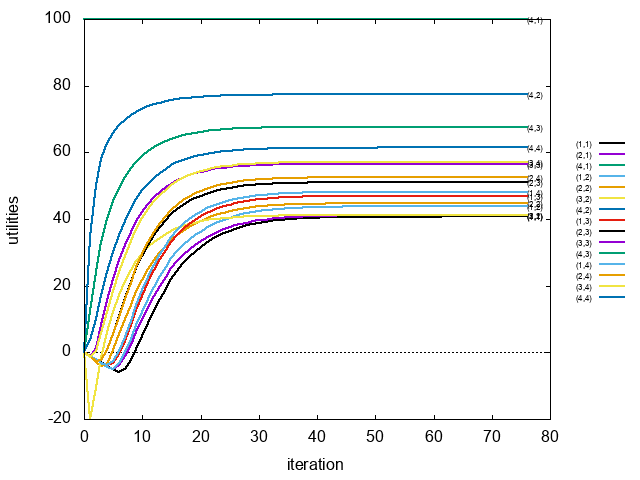
\includegraphics[width=0.8\textwidth]{../results/default4.png}
	\caption{Convergence plot for 4x4 world, modified action uncertainty model}
	\label{q4}
\end{figure}

It takes much longer to achieve stable utility values.

\subsection{World 2 with modifications -- discounting factor}

The discounting factor $\gamma$ was changed to $0.75$. The world is defined in the file \texttt{worlds/default5.toml}.

\begin{lstlisting}[caption={Results of MDP utility value calculation for 4x4 world, modified discounting factor}]
---------------------------------
|>     N|>     N|>     N|v     N|
|8.52018|13.3904|20.0277|28.9742|
---------------------------------
|>     N|>     N|>     N|v     N|
|11.2919|18.2602|28.5480|43.8318|
---------------------------------
|>     N|>     N|>     B|v     N|
|9.29066|15.0289|23.2913|65.6722|
---------------------------------
|^     S|^     N|x     F|x     T|
|5.68543|9.12839|xxxxxxx|    100|
---------------------------------
\end{lstlisting}

The policy slightly changed and now allows to pass through the field with bigger penalty than regular fields have. Utility values are generally much smaller.

\begin{figure}[H]
\centering
	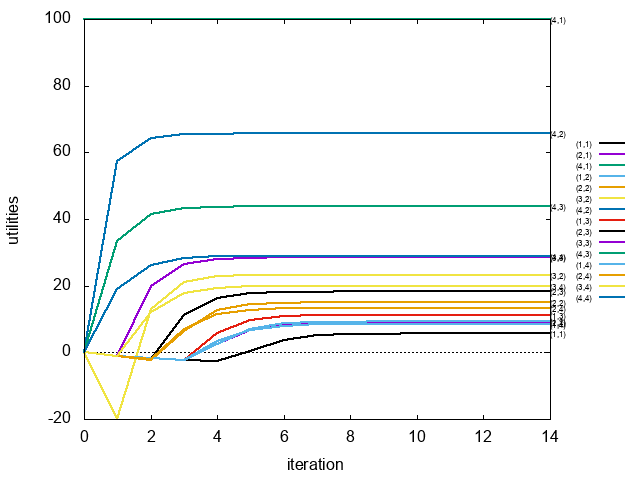
\includegraphics[width=0.8\textwidth]{../results/default5.png}
	\caption{Convergence plot for 4x4 world, modified discounting factor}
	\label{q5}
\end{figure}

Utilities converge to stable values quicker than with higher $\gamma$ (14 iterations). Smaller utility values suggest that the "agent" would not seek to gain a reward in the terminal state as much. Also, allowing to pass through the special state with higher penalty for the move suggests that agent "cares" less about the final reward sum when $\gamma$ is smaller.

\section{Q-learning algorithm}\label{sec_qlearn}

In this task the following calculations were performed:
\begin{itemize}
	\item Q-learning for $\epsilon = 0.2$ (file: \texttt{worlds/default2q02.toml}): 
	\begin{itemize}
		\item 10 000 trails
		\item 100 000 trails
		\item 1 000 000 trails
	\end{itemize}
	\item Q-learning for $\epsilon = 0.05$ (file: \texttt{worlds/default2q005.toml}):
	\begin{itemize}
		\item 10 000 trails
		\item 100 000 trails
		\item 1 000 000 trails
	\end{itemize}
\end{itemize}

The results are listed in listings below. Q-values and policy for each field are listed in the following order: Q-value up, Q-value left, Q-value right, Q-value down, policy. 

Observations:
\begin{itemize}
\item results are closest to those from MDP where 1 000 000 iterations were performed and $\epsilon=0.2$,
\item policies from MDP and Q-learning with 1 000 000 iterations are the same,
\item policies from Q-learning with 100 000 iterations are different for some fields, but Q-values of MDP solver selected action and Q-learning selected action differ slightly,
\item At the same number of iterations, results are better (differ less from MDP-solved solution) with $\epsilon=0.2$.
\end{itemize}


\begin{lstlisting}[float,floatplacement=H,caption={Q-learning: 10 000 iterations, $\epsilon$: 0.2}]
-----------------------------
|^20.63|^35.75|^51.31|^62.42|
|<15.99|<21.15|<39.39|<49.49|
|>35.29|>44.20|>68.69|>59.47|
|v25.95|v51.59|v47.57|v79.20|
|  >   |  v   |  >   |  v   |
-----------------------------
|^21.48|^38.75|^58.30|^70.32|
|<32.52|<37.63|<54.83|<73.33|
|>48.66|>65.82|>78.64|>81.43|
|v37.01|v52.86|v63.17|v88.28|
|  >   |  >   |  >   |  v   |
-----------------------------
|^30.22|^53.94|^51.60|^82.49|
|<42.88|<46.55|<40.28|<68.90|
|>53.45|>62.27|>68.02|>90.60|
|v38.47|v46.33|v47.01|v93.95|
|  >   |  >   |  >   |  v   |
-----------------------------
|^45.28|^54.20|^xxxxx|^  100|
|<35.84|<35.97|<xxxxx|<  100|
|>44.46|>45.23|>xxxxx|>  100|
|v35.75|v42.84|vxxxxx|v  100|
|  ^   |  ^   |  x   |  x   |
-----------------------------
\end{lstlisting}

\begin{lstlisting}[float,floatplacement=H,caption={Q-learning: 10 000 iterations, $\epsilon$: 0.05}]
-----------------------------
|^6.979|^19.77|^37.01|^51.96|
|<2.848|<1.949|<30.93|<41.56|
|>12.91|>44.22|>61.73|>51.73|
|v27.03|v14.41|v48.67|v74.48|
|  v   |  >   |  >   |  v   |
-----------------------------
|^13.23|^30.51|^51.77|^62.31|
|<21.29|<28.21|<43.42|<64.13|
|>41.25|>60.03|>75.58|>77.62|
|v25.64|v38.74|v59.66|v86.90|
|  >   |  >   |  >   |  v   |
-----------------------------
|^27.09|^37.34|^52.04|^80.46|
|<31.43|<32.53|<34.69|<57.86|
|>52.95|>61.18|>67.25|>89.94|
|v21.81|v39.57|v32.45|v93.66|
|  >   |  >   |  >   |  v   |
-----------------------------
|^38.22|^49.80|^xxxxx|^  100|
|<22.22|<9.334|<xxxxx|<  100|
|>27.81|>14.51|>xxxxx|>  100|
|v22.32|v23.02|vxxxxx|v  100|
|  ^   |  ^   |  x   |  x   |
-----------------------------
\end{lstlisting}

\begin{lstlisting}[float,floatplacement=H,caption={Q-learning: 100 000 iterations, $\epsilon$: 0.2}]
-----------------------------
|^35.77|^55.11|^69.24|^78.03|
|<39.46|<42.82|<60.29|<72.75|
|>53.05|>68.32|>78.36|>80.09|
|v47.72|v64.00|v76.31|v84.69|
|  >   |  >   |  >   |  v   |
-----------------------------
|^35.58|^59.65|^71.81|^80.27|
|<53.45|<56.09|<68.48|<80.46|
|>65.11|>75.09|>83.54|>86.78|
|v54.48|v62.18|v68.92|v90.23|
|  >   |  >   |  >   |  v   |
-----------------------------
|^57.06|^62.64|^60.24|^85.69|
|<52.98|<55.28|<45.64|<71.89|
|>60.06|>65.99|>69.31|>92.17|
|v47.13|v55.40|v50.02|v94.25|
|  >   |  >   |  >   |  v   |
-----------------------------
|^53.01|^59.90|^xxxxx|^  100|
|<45.28|<47.10|<xxxxx|<  100|
|>52.93|>54.40|>xxxxx|>  100|
|v45.54|v52.79|vxxxxx|v  100|
|  ^   |  ^   |  x   |  x   |
-----------------------------
\end{lstlisting}

\begin{lstlisting}[float,floatplacement=H,caption={Q-learning: 100 000 iterations, $\epsilon$: 0.05}]
-----------------------------
|^24.04|^45.22|^62.29|^47.00|
|<25.17|<39.99|<54.89|<70.90|
|>55.88|>66.23|>59.16|>16.88|
|v34.51|v58.80|v75.91|v50.20|
|  >   |  >   |  v   |  <   |
-----------------------------
|^43.22|^40.53|^70.93|^67.15|
|<49.61|<54.53|<68.97|<79.00|
|>67.04|>77.10|>84.12|>85.77|
|v50.68|v61.42|v69.18|v90.68|
|  >   |  >   |  >   |  v   |
-----------------------------
|^57.08|^65.04|^61.17|^86.24|
|<53.72|<55.67|<46.11|<72.08|
|>60.76|>66.60|>69.61|>92.17|
|v48.18|v56.39|v50.25|v94.38|
|  >   |  >   |  >   |  v   |
-----------------------------
|^54.09|^60.58|^xxxxx|^  100|
|<46.87|<48.19|<xxxxx|<  100|
|>52.54|>52.80|>xxxxx|>  100|
|v47.12|v51.63|vxxxxx|v  100|
|  ^   |  ^   |  x   |  x   |
-----------------------------
\end{lstlisting}


\begin{lstlisting}[float,floatplacement=H,caption={Q-learning: 1 000 000 iterations, $\epsilon$: 0.2}]
-----------------------------
|^77.91|^80.83|^83.86|^86.23|
|<77.52|<77.89|<81.64|<84.72|
|>80.50|>83.42|>86.07|>86.78|
|v75.35|v79.17|v83.94|v88.55|
|  >   |  >   |  >   |  v   |
-----------------------------
|^78.00|^80.62|^83.98|^86.53|
|<76.98|<76.84|<79.81|<85.56|
|>80.01|>83.28|>86.71|>89.37|
|v74.71|v76.58|v71.70|v91.39|
|  >   |  >   |  >   |  v   |
-----------------------------
|^77.09|^78.37|^65.24|^87.58|
|<72.42|<71.85|<56.33|<73.46|
|>72.78|>68.46|>70.28|>92.71|
|v67.78|v68.94|v52.48|v94.47|
|  ^   |  ^   |  >   |  v   |
-----------------------------
|^71.63|^73.74|^xxxxx|^  100|
|<66.75|<67.00|<xxxxx|<  100|
|>69.54|>69.98|>xxxxx|>  100|
|v66.46|v69.09|vxxxxx|v  100|
|  ^   |  ^   |  x   |  x   |
-----------------------------
\end{lstlisting}

\begin{lstlisting}[float,floatplacement=H,caption={Q-learning: 1 000 000 iterations, $\epsilon$: 0.05}]
-----------------------------
|^72.67|^78.07|^83.00|^86.16|
|<72.29|<73.79|<79.32|<84.64|
|>77.68|>82.47|>86.11|>86.71|
|v74.91|v79.09|v82.10|v88.60|
|  >   |  >   |  >   |  v   |
-----------------------------
|^73.74|^78.62|^82.77|^86.37|
|<74.22|<74.97|<78.83|<85.37|
|>78.36|>82.83|>86.67|>89.40|
|v72.31|v75.26|v71.57|v91.42|
|  >   |  >   |  >   |  v   |
-----------------------------
|^74.71|^78.16|^64.19|^87.54|
|<68.93|<67.24|<52.36|<73.51|
|>64.93|>68.22|>70.23|>92.76|
|v63.55|v63.99|v52.10|v94.50|
|  ^   |  ^   |  >   |  v   |
-----------------------------
|^67.72|^69.55|^xxxxx|^  100|
|<62.06|<61.54|<xxxxx|<  100|
|>64.28|>64.13|>xxxxx|>  100|
|v61.57|v62.90|vxxxxx|v  100|
|  ^   |  ^   |  x   |  x   |
-----------------------------
\end{lstlisting}

\end{document}